% inspired from: https://github.com/SnipyJulmy/hesso-latextemplate-lab
\documentclass[11pt,a4paper,oneside]{report}
\usepackage[margin=2cm]{geometry}
\usepackage[utf8]{inputenc}
\usepackage[T1]{fontenc}
\usepackage[french]{babel}
\usepackage{minted}
\usepackage{titlesec}
\usepackage[pdftex]{graphicx} % graphics importing
\usepackage{titling} % can use \theauthor \thetitle
\usepackage{parskip} % remove first line indenting in a section
\usepackage{microtype} % typographic improvements
\usepackage[defaultlines=3,all]{nowidow}
\usepackage[toc,page]{appendix}
\usepackage{verbatim}

% Header and Footer
\usepackage{fancyhdr}
\pagestyle{fancyplain}
\fancyhf{}
\setlength\headheight{14pt}
\lhead[]{Docker and Embedded systems}
\chead[]{}
\rhead{
\includegraphics[width=3cm]{img/mse_logo}}
\cfoot[]{\thepage}
\renewcommand{\headrulewidth}{0.4pt}% Default \headrulewidth is 0.4pt
\renewcommand{\footrulewidth}{0.4pt}% default is 0pt

\usepackage[hyphens]{url} % line wrap urls
\usepackage{hyperref}

\newminted{bash}{xleftmargin=20pt, linenos=true, breaklines=true, frame=single, framesep=6pt, tabsize=2, fontfamily=courier, fontsize=\small}

% Chapter titles
% Remove space before title
\titlespacing{\chapter}{0pt}{*-4}{*3}
% Remove "Chapter N" and use a sans-serif font
\titleformat{\chapter}{\normalfont\huge}{\thechapter.}{20pt}{\huge}
% Change chapter page style
\patchcmd{\chapter}{plain}{fancy}{}{}

\title{État de l'art à la mi-projet de semestre Docker and embedded systems - Où comment ne pas cross compiler Docker sur ARM}
\author{Gary \bsc{Marigliano}}

\begin{document}

\begin{titlepage}
  \centering
  \vfill
  \LARGE \thetitle\\[0.8cm]

  \Large \theauthor\\[0.8cm]

  \normalsize \today
  \vfill
  
\includegraphics[width=8cm]{img/docker_logo}
  \vfill
\end{titlepage}

\pagenumbering{gobble}
\tableofcontents
\pagenumbering{arabic}

\chapter{Introduction}

\section{Contexte}\label{contexte}

Ce document s'inscrit dans le cadre du projet de semestre Docker and embedded systems actuellement réalisé par moi-même. Un des buts de ce projet est de cross-compiler Docker à partir de ses sources pour produire un binaire exécutable sur un Odroid XU3 (ARMv7).

Lien: \url{https://github.com/krypty/docker_and_embedded_systems}

Il est important de noter que la vitesse de développement de Docker est assez hallucinante. En effet, sur Github (\url{https://github.com/docker/docker}) les commits se succèdent à vitesse grand V. Entre chaque version de Docker qui sortent environ tous les mois, il est courant d'avoir plus de 3000 commits qui ont été \emph{pushés}. Tout ceci pour dire qu'à la lecture de ce document, il est quasiment sûr que certaines pistes explorées soient définitivement obsolètes ou au contraire deviennent la voie à suivre du à une mise à jour quelconque.


\section{Objectifs}

De manière plus précise, ce projet vise à maitriser les parties suivantes:

\begin{enumerate}
  \item Construction d'un système Linux capable de faire tourner Docker et son \emph{daemon} en utilisant Buildroot. Pour générer le dit système, on dispose d'un \emph{repository} Gitlab hébergé à la Haute École de Fribourg.

  \item Cross-compilation de Docker et de son \emph{daemon}, capable de faire tourner des containers
\end{enumerate}

L'objectif de ce document est d'énumérer les différentes techniques tentées pour (cross-)compiler Docker sur une cible ARM. De cette manière, le lecteur, en cas de reprise du projet ou par simple curiosité, aura une idée des pistes à explorer ou à éviter.



\chapter{Objectif 1 - Construction d'un système GNU/Linux Docker-ready}

Dans cette partie, on verra les ingrédients et pistes à suivre pour concevoir un système construit à partir de Buildroot capable de faire tourner Docker et son \emph{daemon}.

\section{Générer le système}

Comme évoqué à la section \ref{contexte}, on dispose d'un Odroid XU3 sur lequel il faut générer un système GNU/Linux. Dans le cadre d'un cours, la Haute École de Fribourg met à disposition un \emph{repository} git qui contient tout ce qu'il faut pour gérérer un tel système.

Toutes les ressources nécessaires à la génération du système se trouvent ici :

\begin{itemize}
  \item Procédure de génération du système du cours CSEL : \emph{\newline p.02.2\_mas\_csel\_environnement\_linux\_embarque\_exercices.pdf}
  \item Script de génération de la carte utilisé : \url{https://github.com/krypty/docker\_and\_embedded\_systems/blob/master/write\_system\_on\_sd.sh}
  \item Le PDF \emph{01\_IntroOdroidXu3.pdf} du cours SeS
\end{itemize}

Le système généré, ne peut, dans sa configuration actuelle, permettre à Docker de se lancer. Pour pouvoir le faire, on a deux moyens à dispositions : Buildroot et le kernel.

Grossièrement, Buildroot permet d'ajouter des packages et de configurer son système tandis que le kernel permet d'ajouter des modules ou des drivers.

\section{Vérifier que le système peut faire tourner Docker}

Il faut en premier lieu mettre la main sur un binaire ARM Docker qui intègre le \emph{daemon}. En effet, à l'heure actuelle, lorsqu'on compile Docker pour ARM de la manière officielle, le binaire résultant n'intègre pas le \emph{daemon} mais uniquement le client (qui permet de se connecter à un \emph{daemon} externe). Voir également à la section \ref{maniere_officielle_limitations}

Le seul binaire de ce type que j'ai trouvé actuellement est téléchargeable ici: \url{https://github.com/umiddelb/armhf/raw/master/bin/docker-1.9.1}.

Copiez ce fichier sur la cible et tentez de le lancer avec:

\begin{bashcode}
chmod +x docker-1.9.1
./docker-1.9.1 deamon
\end{bashcode}

S'il y a des erreurs c'est sûrement qu'il manque un ou plusieurs modules kernel. Pour vérifier que la configuration actuelle du noyau est correcte. L'équipe Docker met à disposition un script qui indique quels modules sont manquants.

Ce script est à télécharger ici: \url{https://github.com/docker/docker/blob/master/contrib/check-config.sh}

\newpage
Voici un exemple de sortie où l'on voit qu'il manque certains modules:

\begin{bashcode}
/ # ./check-config.sh
info: reading kernel config from /proc/config.gz ...

Generally Necessary:
- cgroup hierarchy: nonexistent??
    (see https://github.com/tianon/cgroupfs-mount)
- CONFIG_NAMESPACES: enabled
- CONFIG_NET_NS: enabled
- CONFIG_PID_NS: enabled
- CONFIG_IPC_NS: enabled
- CONFIG_UTS_NS: enabled
- CONFIG_DEVPTS_MULTIPLE_INSTANCES: missing
- CONFIG_CGROUPS: enabled
- CONFIG_CGROUP_CPUACCT: enabled
- CONFIG_CGROUP_DEVICE: enabled
- CONFIG_CGROUP_FREEZER: enabled
- CONFIG_CGROUP_SCHED: missing
...
- CONFIG_NETFILTER_XT_MATCH_CONNTRACK: missing
- CONFIG_NF_NAT: missing
- CONFIG_NF_NAT_NEEDED: missing
- CONFIG_POSIX_MQUEUE: enabled

Optional Features:
- CONFIG_USER_NS: missing
- CONFIG_SECCOMP: enabled
- CONFIG_CGROUP_PIDS: missing
- CONFIG_MEMCG_KMEM: enabled
...
- CONFIG_EXT3_FS: enabled
- CONFIG_EXT3_FS_XATTR: missing
- CONFIG_EXT3_FS_POSIX_ACL: enabled
- CONFIG_EXT3_FS_SECURITY: enabled
    (enable these ext3 configs if you are using ext3 as backing filesystem)
- CONFIG_EXT4_FS: enabled
- CONFIG_EXT4_FS_POSIX_ACL: enabled
- CONFIG_EXT4_FS_SECURITY: enabled
- Storage Drivers:
  - "aufs":
    - CONFIG_AUFS_FS: missing
  - "btrfs":
    - CONFIG_BTRFS_FS: enabled (as module)
  - "devicemapper":
    - CONFIG_BLK_DEV_DM: enabled
    - CONFIG_DM_THIN_PROVISIONING: missing
  - "overlay":
    - CONFIG_OVERLAY_FS: enabled (as module)
  - "zfs":
    - /dev/zfs: missing
    - zfs command: missing
    - zpool command: missing
\end{bashcode}

La suite consiste à modifier le kernel pour y ajouter les modules manquants, de reflasher le système et tester à nouveau si Docker se lance.

Je n'explique volontairement pas comment modifier la configuration d'un kernel Linux, car d'une part cette information se trouve facilement sur internet ou sur les documents indiqués plus haut et d'autre une car ce n'est pas le but de ce rapport.

\chapter{Objectif 2 - Techniques de compilation essayées}

\section{La manière officielle}\label{maniere_officielle}

C'est la manière recommandée et qui, un jour, sera celle qu'il faudra
employer. Mais aujourd'hui, elle ne permet que de cross compiler un
binaire ARM Docker qui n'embarque pas le \emph{deamon}.

\subsection{Principe utilisé}

Pour compiler Docker de la manière officiellement supportée, on doit utiliser Docker. En effet, le Makefile fourni va lancer un container Docker qui va contenir un système d'exploitation ainsi que tous les pré-requis et dépendances puis lancer la compilation de Docker à l'intérieur de ce container.

\subsection{Cheminement général}

Sur une machine GNU/Linux

\begin{bashcode}
git clone https://github.com/docker/docker
cd docker
git checkout v1.10.3 -b tmp_build # vous pouvez remplacez v1.10.3 par la dernière version (tag) stable
make build
make binary # pour générer le binaire sur la plateforme sur laquelle on est en train de compiler (probablement x64)
make cross # pour générer le binaire ARM
\end{bashcode}

Le binaire se trouve dans le dossier ./bundle.

\subsection{Schéma}

Comme on peut le voir à la figure \ref{fig_docker_in_docker}, pour compiler Docker, il faut disposer de Docker sur son PC. En faisant une commande \textit{make}, Docker va créer un container basé sur une image Ubuntu et va installer tous les outils de compilation nécessaires. Une fois que cela est fait, Docker utilise ce container pour lancer la compilation. Le binaire est ensuite récupéré dans le dossier \textit{./bundle}. Il ne reste plus qu'à copier le binaire sur la cible.

\begin{figure}
    \begin{center}
        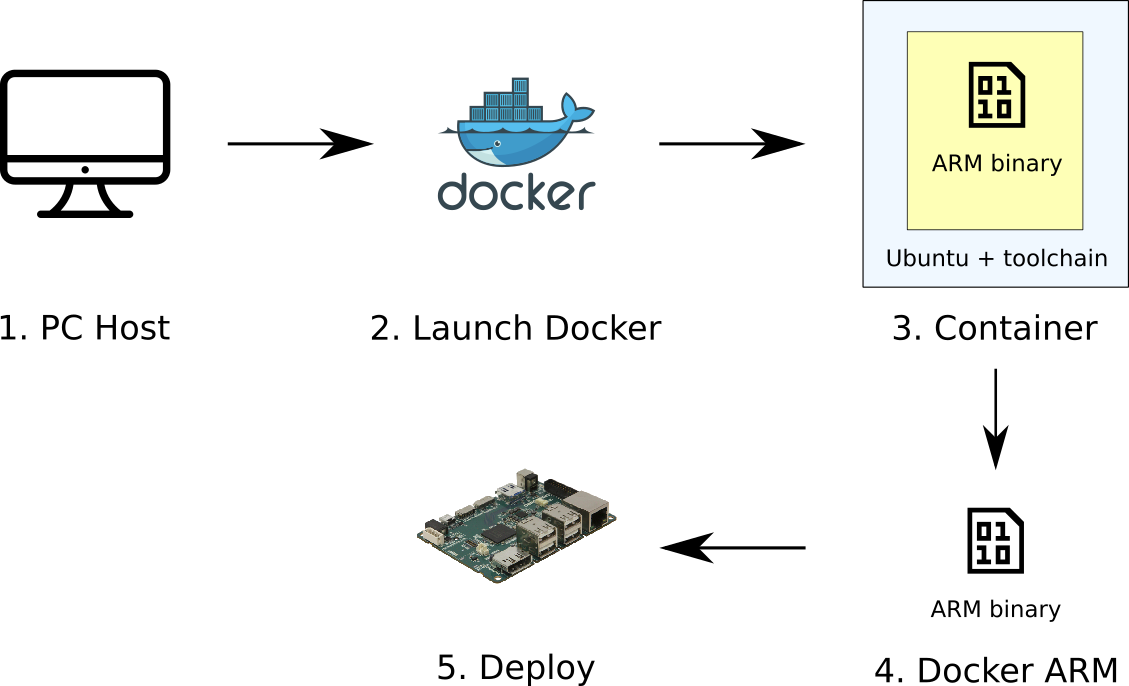
\includegraphics[scale=0.6]{img/docker_in_docker}
    \end{center}
    \caption{Docker in Docker}
    \label{fig_docker_in_docker}
\end{figure}

\subsection{Limitations}\label{maniere_officielle_limitations}

Actuellement, il est possible de générer un binaire Docker x64 et ARM mais seule l'architecture x64 intègre le \emph{deamon} nécessaire à la création de containers.

Le binaire ARM est dit CLIENT\_ONLY dans le sens où il peut être le client d'un \emph{deamon} Docker remote (instancié sur une autre machine).



\section{Compiler directement sur une machine ARM en utilisant la manière officielle}

Il existe certaines limitations.
Il existe certaines limitations.
Il existe certaines limitations.
Il existe certaines limitations.
Il existe certaines limitations.
Il existe certaines limitations.
Il existe certaines limitations.
Il existe certaines limitations.
Il existe certaines limitations.
Il existe certaines limitations.
Il existe certaines limitations.
Il existe certaines limitations.
\subsection{Principe utilisé}

Il existe certaines limitations.
Il existe certaines limitations.
Il existe certaines limitations.
Il existe certaines limitations.
Il existe certaines limitations.
Il existe certaines limitations.
Il existe certaines limitations.
Il existe certaines limitations.
Il existe certaines limitations.
Il existe certaines limitations.
Il existe certaines limitations.
Il existe certaines limitations.
\subsection{Cheminement général}

Il existe certaines limitations.
Il existe certaines limitations.
Il existe certaines limitations.
Il existe certaines limitations.
Il existe certaines limitations.
Il existe certaines limitations.
Il existe certaines limitations.
Il existe certaines limitations.
Il existe certaines limitations.
Il existe certaines limitations.
Il existe certaines limitations.
Il existe certaines limitations.
\subsection{Schéma}

Il existe certaines limitations.
Il existe certaines limitations.
Il existe certaines limitations.
Il existe certaines limitations.
Il existe certaines limitations.
Il existe certaines limitations.
Il existe certaines limitations.
Il existe certaines limitations.
Il existe certaines limitations.
Il existe certaines limitations.
Il existe certaines limitations.
Il existe certaines limitations.
\subsection{Limitations}

Il existe certaines limitations.
Il existe certaines limitations.
Il existe certaines limitations.
Il existe certaines limitations.
Il existe certaines limitations.
Il existe certaines limitations.
Il existe certaines limitations.
Il existe certaines limitations.
Il existe certaines limitations.
Il existe certaines limitations.
Il existe certaines limitations.
Il existe certaines limitations.


\section{Compiler en émulant une machine ARM sur un PC de bureau avec QEMU et chroot}

Il existe certaines limitations.
Il existe certaines limitations.
Il existe certaines limitations.
Il existe certaines limitations.
Il existe certaines limitations.
Il existe certaines limitations.
Il existe certaines limitations.
Il existe certaines limitations.
Il existe certaines limitations.
Il existe certaines limitations.
Il existe certaines limitations.
Il existe certaines limitations.
\subsection{Principe utilisé}

Il existe certaines limitations.
Il existe certaines limitations.
Il existe certaines limitations.
Il existe certaines limitations.
Il existe certaines limitations.
Il existe certaines limitations.
Il existe certaines limitations.
Il existe certaines limitations.
Il existe certaines limitations.
Il existe certaines limitations.
Il existe certaines limitations.
Il existe certaines limitations.
\subsection{Cheminement général}

Il existe certaines limitations.
Il existe certaines limitations.
Il existe certaines limitations.
Il existe certaines limitations.
Il existe certaines limitations.
Il existe certaines limitations.
Il existe certaines limitations.
Il existe certaines limitations.
Il existe certaines limitations.
Il existe certaines limitations.
Il existe certaines limitations.
Il existe certaines limitations.
\subsection{Schéma}

Il existe certaines limitations.
Il existe certaines limitations.
Il existe certaines limitations.
Il existe certaines limitations.
Il existe certaines limitations.
Il existe certaines limitations.
Il existe certaines limitations.
Il existe certaines limitations.
Il existe certaines limitations.
Il existe certaines limitations.
Il existe certaines limitations.
Il existe certaines limitations.
\subsection{Limitations}

Il existe certaines limitations.
Il existe certaines limitations.
Il existe certaines limitations.
Il existe certaines limitations.
Il existe certaines limitations.
Il existe certaines limitations.
Il existe certaines limitations.
Il existe certaines limitations.
Il existe certaines limitations.
Il existe certaines limitations.
Il existe certaines limitations.
Il existe certaines limitations.


\section{Compiler en émulant une machine ARM sur un PC de bureau avec QEMU et une image Debian}

Il existe certaines limitations.
Il existe certaines limitations.
Il existe certaines limitations.
Il existe certaines limitations.
Il existe certaines limitations.
Il existe certaines limitations.
Il existe certaines limitations.
Il existe certaines limitations.
Il existe certaines limitations.
Il existe certaines limitations.
Il existe certaines limitations.
Il existe certaines limitations.
\subsection{Principe utilisé}

Il existe certaines limitations.
Il existe certaines limitations.
Il existe certaines limitations.
Il existe certaines limitations.
Il existe certaines limitations.
Il existe certaines limitations.
Il existe certaines limitations.
Il existe certaines limitations.
Il existe certaines limitations.
Il existe certaines limitations.
Il existe certaines limitations.
Il existe certaines limitations.
\subsection{Cheminement général}

Il existe certaines limitations.
Il existe certaines limitations.
Il existe certaines limitations.
Il existe certaines limitations.
Il existe certaines limitations.
Il existe certaines limitations.
Il existe certaines limitations.
Il existe certaines limitations.
Il existe certaines limitations.
Il existe certaines limitations.
Il existe certaines limitations.
Il existe certaines limitations.
\subsection{Schéma}

Il existe certaines limitations.
Il existe certaines limitations.
Il existe certaines limitations.
Il existe certaines limitations.
Il existe certaines limitations.
Il existe certaines limitations.
Il existe certaines limitations.
Il existe certaines limitations.
Il existe certaines limitations.
Il existe certaines limitations.
Il existe certaines limitations.
Il existe certaines limitations.
\subsection{Limitations}

Il existe certaines limitations.
Il existe certaines limitations.
Il existe certaines limitations.
Il existe certaines limitations.
Il existe certaines limitations.
Il existe certaines limitations.
Il existe certaines limitations.
Il existe certaines limitations.
Il existe certaines limitations.
Il existe certaines limitations.
Il existe certaines limitations.
Il existe certaines limitations.



\section{Compiler en émulant une machine ARM sur un PC de bureau avec QEMU et une image Raspbian}

Il existe certaines limitations.
Il existe certaines limitations.
Il existe certaines limitations.
Il existe certaines limitations.
Il existe certaines limitations.
Il existe certaines limitations.
Il existe certaines limitations.
Il existe certaines limitations.
Il existe certaines limitations.
Il existe certaines limitations.
Il existe certaines limitations.
Il existe certaines limitations.
\subsection{Principe utilisé}

Il existe certaines limitations.
Il existe certaines limitations.
Il existe certaines limitations.
Il existe certaines limitations.
Il existe certaines limitations.
Il existe certaines limitations.
Il existe certaines limitations.
Il existe certaines limitations.
Il existe certaines limitations.
Il existe certaines limitations.
Il existe certaines limitations.
Il existe certaines limitations.
\subsection{Cheminement général}

Il existe certaines limitations.
Il existe certaines limitations.
Il existe certaines limitations.
Il existe certaines limitations.
Il existe certaines limitations.
Il existe certaines limitations.
Il existe certaines limitations.
Il existe certaines limitations.
Il existe certaines limitations.
Il existe certaines limitations.
Il existe certaines limitations.
Il existe certaines limitations.
\subsection{Schéma}

Il existe certaines limitations.
Il existe certaines limitations.
Il existe certaines limitations.
Il existe certaines limitations.
Il existe certaines limitations.
Il existe certaines limitations.
Il existe certaines limitations.
Il existe certaines limitations.
Il existe certaines limitations.
Il existe certaines limitations.
Il existe certaines limitations.
Il existe certaines limitations.
\subsection{Limitations}

Il existe certaines limitations.
Il existe certaines limitations.
Il existe certaines limitations.
Il existe certaines limitations.
Il existe certaines limitations.
Il existe certaines limitations.
Il existe certaines limitations.
Il existe certaines limitations.
Il existe certaines limitations.
Il existe certaines limitations.
Il existe certaines limitations.
Il existe certaines limitations.


\section{Compiler en émulant une machine ARM sur un PC de bureau avec QEMU et une image Archlinux ARM}

Il existe certaines limitations.
Il existe certaines limitations.
Il existe certaines limitations.
Il existe certaines limitations.
Il existe certaines limitations.
Il existe certaines limitations.
Il existe certaines limitations.
Il existe certaines limitations.
Il existe certaines limitations.
Il existe certaines limitations.
Il existe certaines limitations.
Il existe certaines limitations.
\subsection{Principe utilisé}

Il existe certaines limitations.
Il existe certaines limitations.
Il existe certaines limitations.
Il existe certaines limitations.
Il existe certaines limitations.
Il existe certaines limitations.
Il existe certaines limitations.
Il existe certaines limitations.
Il existe certaines limitations.
Il existe certaines limitations.
Il existe certaines limitations.
Il existe certaines limitations.

\subsection{Cheminement général}

Il existe certaines limitations.
Il existe certaines limitations.
Il existe certaines limitations.
Il existe certaines limitations.
Il existe certaines limitations.
Il existe certaines limitations.
Il existe certaines limitations.
Il existe certaines limitations.
Il existe certaines limitations.
Il existe certaines limitations.
Il existe certaines limitations.
Il existe certaines limitations.
\subsection{Schéma}

Il existe certaines limitations.
Il existe certaines limitations.
Il existe certaines limitations.
Il existe certaines limitations.
Il existe certaines limitations.
Il existe certaines limitations.
Il existe certaines limitations.
Il existe certaines limitations.
Il existe certaines limitations.
Il existe certaines limitations.
Il existe certaines limitations.
Il existe certaines limitations.
\subsection{Limitations}

Il existe certaines limitations.
Il existe certaines limitations.
Il existe certaines limitations.
Il existe certaines limitations.
Il existe certaines limitations.
Il existe certaines limitations.
Il existe certaines limitations.
Il existe certaines limitations.
Il existe certaines limitations.
Il existe certaines limitations.
Il existe certaines limitations.
Il existe certaines limitations.
Il existe certaines limitations.
Il existe certaines limitations.
Il existe certaines limitations.
Il existe certaines limitations.
Il existe certaines limitations.
Il existe certaines limitations.


\section{Compiler Docker sans Docker}

Il existe certaines limitations.
Il existe certaines limitations.
Il existe certaines limitations.
Il existe certaines limitations.
Il existe certaines limitations.
Il existe certaines limitations.
Il existe certaines limitations.
Il existe certaines limitations.
Il existe certaines limitations.
Il existe certaines limitations.
Il existe certaines limitations.
Il existe certaines limitations.
Il existe certaines limitations.
Il existe certaines limitations.
Il existe certaines limitations.
Il existe certaines limitations.
Il existe certaines limitations.
Il existe certaines limitations.
\subsection{Principe utilisé}

Il existe certaines limitations.
Il existe certaines limitations.
Il existe certaines limitations.
Il existe certaines limitations.
Il existe certaines limitations.
Il existe certaines limitations.
Il existe certaines limitations.
Il existe certaines limitations.
Il existe certaines limitations.
Il existe certaines limitations.
Il existe certaines limitations.
Il existe certaines limitations.
Il existe certaines limitations.
Il existe certaines limitations.
Il existe certaines limitations.
Il existe certaines limitations.
Il existe certaines limitations.
Il existe certaines limitations.
\subsection{Cheminement général}

Il existe certaines limitations.
Il existe certaines limitations.
Il existe certaines limitations.
Il existe certaines limitations.
Il existe certaines limitations.
Il existe certaines limitations.
Il existe certaines limitations.
Il existe certaines limitations.
Il existe certaines limitations.
Il existe certaines limitations.
Il existe certaines limitations.
Il existe certaines limitations.
Il existe certaines limitations.
Il existe certaines limitations.
Il existe certaines limitations.
Il existe certaines limitations.
Il existe certaines limitations.
Il existe certaines limitations.
\subsection{Schéma}

Il existe certaines limitations.
Il existe certaines limitations.
Il existe certaines limitations.
Il existe certaines limitations.
Il existe certaines limitations.
Il existe certaines limitations.
Il existe certaines limitations.
Il existe certaines limitations.
Il existe certaines limitations.
Il existe certaines limitations.
Il existe certaines limitations.
Il existe certaines limitations.
Il existe certaines limitations.
Il existe certaines limitations.
Il existe certaines limitations.
Il existe certaines limitations.
Il existe certaines limitations.
Il existe certaines limitations.
\subsection{Limitations}

Il existe certaines limitations.
Il existe certaines limitations.
Il existe certaines limitations.
Il existe certaines limitations.
Il existe certaines limitations.
Il existe certaines limitations.
Il existe certaines limitations.
Il existe certaines limitations.
Il existe certaines limitations.
Il existe certaines limitations.
Il existe certaines limitations.
Il existe certaines limitations.
Il existe certaines limitations.
Il existe certaines limitations.
Il existe certaines limitations.
Il existe certaines limitations.
Il existe certaines limitations.
Il existe certaines limitations.

\begin{appendices}
  \chapter{Script : Write system on SD}

  \inputminted[xleftmargin=20pt, linenos=true, breaklines=true, frame=single, framesep=6pt, tabsize=2, fontfamily=courier, fontsize=\small]{bash}{../write_system_on_sd.sh}

\end{appendices}
\end{document}
